\capitulo{3}{Conceptos teóricos}

Para la correcta comprensión del proyecto se van a explicar a continuación una serie de conceptos teóricos mínimos necesarios.

\section{Micología}

La micología es la ciencia que se dedica al estudio de los hongos. Es una de las áreas de la ciencia más extensas y diversificadas que aporta avances significativos a la investigación científica y al desarrollo tecnológico. ~\cite{wiki:micologia}

Tiene varios aplicaciones y objetivos, se usa para determinar que especies de hongos son comestibles o no y si podrían usarse para diferentes tratamientos médicos, ciertas sustancias de las setas son estudiadas con estos fines curativos. \cite{micologiaDef}

\section{Hongos}

El hongo es el nombre común de los organismos del reino Fungi. El término Fungi en biología se refiere a un grupo de organismos eucariotas\footnote{Aquellos organismos formados por células con núcleo verdadero} que se clasifican en un reino distinto al de las plantas, animales y protistas. Se diferencian de las plantas en que son heterótrofos\footnote{Seres vivos que necesitan de otros para alimentarse} y de los animales en que tienen paredes celulares, como las plantas, pero compuestas de quitina\footnote{\url{https://es.wikipedia.org/wiki/Quitina}} en vez de celulosa.

Los hongos se reproducen de forma sexual o asexual mediante esporas, que se dispersan en un estado latente y solo se interrumpe cuando se dan las condiciones adecuadas para su germinación. ~\cite{wiki:fungi}

La mayoría de los hongos están formados por estructuras microscópicas, filamentosas y ramificadas llamadas hifas. El conjunto de estas hifas forma una red a la que llamaremos micelio. Cuando la acumulación de hifas es grande se pueden observar como una red algonodosa que se pueden reconocer por ejemplo cuando los alimentos empiezan a descomponerse. ~\cite{setas}

\section{Setas}

Las setas son los cuerpos fructíferos de algunos tipos de hongos (no todos los hongos producen setas), en otras palabras, son la parte reproductiva de los hongos. La principal función de la seta es dispersar las esporas del hongo. Normalmente es la parte visible del hongo ya que este suele estar bajo tierra.

\subsection{Partes de las setas}

A continuación se van a describir las partes más características de una seta que se usan para su clasificación.

\begin{itemize}
	\item{Sombrero}: Situado sobre el pie, ejerce la función de protección en la formación y desarrollo de las esporas. El sombrero es un elemento clave a la hora de diferenciar las especies ya que puede adoptar diferentes formas, aspectos y colores.
	\item{Himenio}: Es la parte situada justo debajo del sobrero y que puede adoptar diferentes formas(láminas, tubos, aguijones o pliegues), estas diferentes formas nos ayudarán a diferenciar entre las especies. La función principal de esta parte es la de crear, desarrollar, almacenar y dispersar las esporas que generan nuevos hongos.
	\item{Pie}: Elemento que no tiene por que aparecer en todas las setas y que sujeta al sombrero e himenio.
	\item{Volva}: Es un fragmento en forma de membrana que envuelve la base del pie en algunas setas. Es un error común cortar el pie de la seta y no conservar la volva que nos podría dar indicios de a que especie pertenece la seta.~\cite{partesSeta}
\end{itemize}

En la siguiente figura \ref{figpartesDeLaSeta} se muestran las partes más relevantes de una seta.

\begin{figure}[h]
    \begin{center}%
        \begin{center}%
          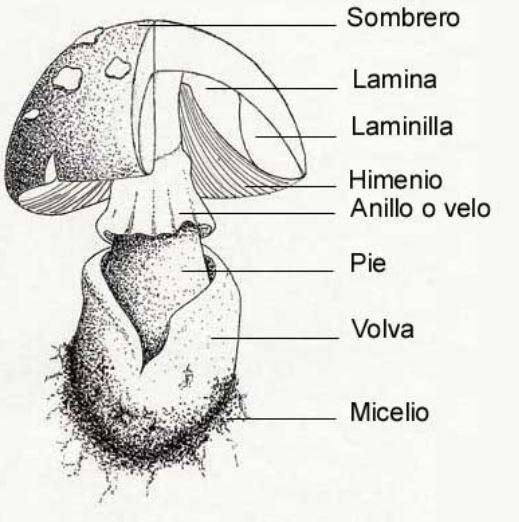
\includegraphics[width=1\textwidth]{partesDeLaSeta}%
          \caption{Partes de una seta}%
          \label{figpartesDeLaSeta}%
        \end{center}%
  	\end{center}%
\end{figure}%

\section{Inteligencia Artificial}
%https://luismejias21.files.wordpress.com/2017/09/inteligencia-artificial-un-enfoque-moderno-stuart-j-russell.pdf
Hay muchas definiciones para definir lo que es la inteligencia artificial, normalmente aparece bajo las siglas IA o AI (Del inglés Artificial Intelligence), pero de forma general la podemos definir como el desarrollo de algoritmos y métodos que otorgan a las computadoras la capacidad de realizar acciones o tareas como las realizaría un ser humano. La inteligencia artificial se aplica en multitud de campos como puede ser la robótica, automovilismo, reconocimiento de imágenes, medicina, sistemas de apoyo...

Stuart Russell y Peter Norving\cite{wiki:tiposInteligenciaArtificial}  diferencian estos cuatro tipos de inteligencia artificial:

\begin{itemize}
	\item{Sistemas que piensan como humanos}: Son sistemas que intentan emular el pensamiento humano automatizando actividades que relacionamos con los procesos de pensamiento humano(toma de decisiones, resolución de problemas...), por ejemplo las redes neuronales artificiales.
	\item{Sistemas que actúan como humanos}: Este tipo de sistemas intentan imitar el comportamiento humano, por ejemplo la robótica.
	\item{Sistemas que piensan racionalmente}: Tratan de imitar con lógica el pensamiento lógico racional del ser humano, por ejemplo los sistemas expertos.
	\item{Sistemas que actúan racionalmente}:Intentan emular de forma racional el comportamiento humano.
\end{itemize}

Algunos de estos sistemas necesitan desarrollar una capacidad de aprendizaje para poder imitar de forma correcta el comportamiento humano.

\subsection{Aprendizaje automático}

El aprendizaje automático (del inglés Machine Learning) es una rama de la inteligencia artificial que se encarga de desarrollar los algoritmos que permitan a las computadoras aprender ~\footnote{Adquirir conocimiento por medio de la experiencia}. Para ello, se entrenan los sistemas con una serie de ejemplos, o información de entrenamiento, para generalizar comportamientos que deben realizar ante diferentes casos de entrada.

Hay una gran variedad de algoritmos de aprendizaje automático, a continuación se presentan algunos de los tipos más extendidos:
\begin{itemize}

	\item{Aprendizaje supervisado}: En estos algoritmos se intenta crear una función que nos de la correspondencia entre los datos de entrada y una de las salidas deseadas. En este tipo de algoritmos se tiene información tanto de los valores de entrada como del los valores deseados.Para entrenar se suelen usar pares en los que un componente son los datos de entrada y otro los valores deseados. Los valores deseados suelen ser denominados como clases.~\cite{wiki:aprendizaheSupervisado}
	
	El valor de salida de la función puede ser un número(Regresión) o una etiqueta de clase(Clasificación).
	
	Los algoritmos de clasificación usados en este proyecto se corresponderían con este tipo de aprendizaje, siendo las etiquetas de clase las especies de setas que se quieren clasificar.
	
	\item{Aprendizaje no supervisado}: El aprendizaje no supervisado se diferencia del supervisado en que no se conoce a priori los resultados deseados. En este tipo de aprendizaje, normalmente, se tratan los datos de entrada como una serie de datos aleatorios y se intentan buscar relaciones ocultas entre ellos.
	Una forma de aprendizaje no supervisado es el clustering, el cuál se encarga de organizar los datos de entrada en grupos en los que comparten propiedades y los diferencian del resto.~\cite{wiki:aprendizajeNoSupervisado}
	
	\item{Aprendizaje semisupervisado}: Este tipo de aprendizaje mezcla las dos técnicas descritas anteriormente. Se usa cuando tenemos tanto datos conocidos como datos de los que no tenemos conocimiento.
	
	\item{Aprendizaje por refuerzo}: Este tipo de algoritmos realiza una aprendizaje mediante el modelo de prueba-error, es decir, el algoritmo realiza acciones y a partir de los resultados de estas el algoritmo evalúa cual han sido beneficiosas y cuales no.
\end{itemize}
	
En nuestro proyecto se hace uso del aprendizaje supervisado para entrenar el clasificador de imágenes que reconocerá las especies de las setas.
~\cite{wiki:aprendizajeAutomatico}

\section{Minería de datos}

La minería de datos consiste en la aplicación de técnicas de inteligencia artificial sobre grandes cantidades de datos con el objetivo de descubrir patrones o relaciones ocultas entre los datos. La parte de la minería de datos más relevante para nuestro proyecto son los clasificadores previamente introducidos \cite{procesosMineriaDatos}. Básicamente los clasificadores se basan en la hipótesis del aprendizaje inductivo:

Cualquier hipótesis que aproxime bien una función objetivo sobre un conjunto de ejemplos de entrenamiento suficientemente grande también aproximará bien la función objetivo en ejemplos no observados //CITAR UBU

La míneria de datos, típicamente, consta de los siguientes pasos:
\begin{itemize}
	\item{Selección del conjunto de datos}: En esta parte del proceso se seleccionarán las variables objetivo, las variables independientes y se realizará un muestreo con los registros disponibles.
	\item{Análisis de las propiedades de los datos}: Se comprobarán los histogramas, diagramas de dispersión, si se encuentran valores atípicos entre el conjunto de datos y si faltan ciertos datos.
	\item{Transformación de los datos}: En esta etapa del proceso se procesarán los datos de entrada para adecuarlos a la estructura requerida por las técnicas de inteligencia artificial que se aplicarán sobre ellos.
	\item{Selección de la técnica de minería de datos}: Se construirá el modelo predictivo a aplicar sobre los datos. Clasificación o segmentación.
	\item{Extracción del conocimiento}: Esta es la parte donde se aplicarán las técnicas de inteligencia artificial sobre los datos para extraer el conocimiento buscado. La técnica que hayamos aplicado nos devolverá un modelo de conocimiento sobre los datos.
	\item{Interpretación y evaluación de los datos}: Esta última etapa consiste en validar si los resultados que nos ofrece el modelo entrenado son satisfactorios y se adecuan a los requisitos pedidos.
\end{itemize}

\subsection{Evolución del flujo de trabajo}

Al principio, el flujo de trabajo para entrenar un clasificador, era el de extraer unas características de los datos de entrenamiento que se proporcionaban al clasificador. En este modo de trabajo se usan métodos como el Bag-of-words\footnote{Por ejemplo, tratar las características de una imágen como palabras y guardar las veces que se repiten estas características en cada imagen. \url{https://es.wikipedia.org/wiki/Modelo_bolsa_de_palabras}} para determinar las características de los datos de entrada.

Posteriormente, este flujo de trabajo se ha modificado, introduciendo redes neuronales que se encargan de extraer estas características y dividiéndolas en diferentes jerarquías para que no todas tengan el mismo peso a la hora de clasificar.

\begin{figure}[h]
    \begin{center}%
        \begin{center}%
          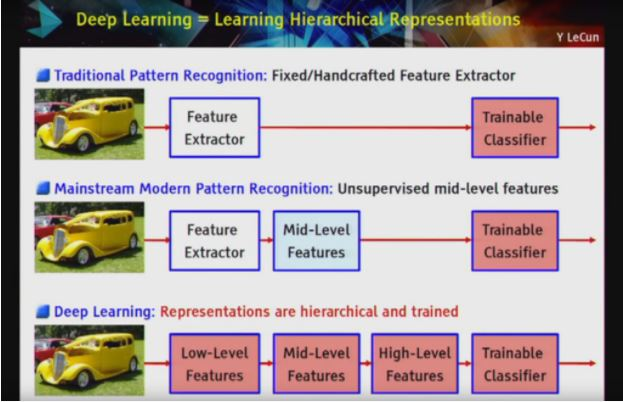
\includegraphics[width=0.7\textwidth]{FlujoTrabajo}%
          \caption{Flujos de trabajo, clasificación}%
          \label{figFlujo}%
        \end{center}%
  	\end{center}%
\end{figure}%

En la figura \ref{figFlujo} se muestra como se han ido incorporando diferentes capas, todas de ellas entrenables, para extraer las características de una forma jerárquica mediante redes neuronales.

\newpage

\section{Redes neuronales}

En esta sección se explicarán algunos conceptos teóricos sobre redes neuronales necesarios para entender el funcionamiento de los modelos Mobilenet e Inception usados para clasificar imágenes en nuestro proyecto. Actualmente hay gran variedad de clasificadores que se pueden usar para esta tarea además de los dos mencionados.

\subsection{Modelo de neurona artificial}

Una neurona artificial de forma general se puede describir según el modelo de Rumelhart y McClelland (1986), el cual define la neurona o elemento de proceso(EP) como un dispostivo el cuál a partir de un conjunto de entradas, vector x, genera una única salida y. \cite{redesNeurnalesUno}

\begin{figure}[h]
    \begin{center}%
        \begin{center}%
          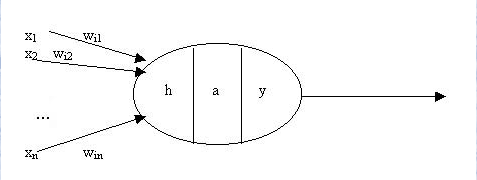
\includegraphics[width=1\textwidth]{modeloNeuronaArtificial}%
          \caption{Modelo de una neurona artificial}%
          \label{figmodeloNeuronaArtificial}%
        \end{center}%
  	\end{center}%
\end{figure}%

\newpage
La neurona artifcial consta de los siguientes elementos:

\begin{itemize}
	\item{Conjunto de entradas x}: El vector x.
	\item{Conjunto de pesos sinápticos wij}: Representan la relación entre la neurona i y j.
	\item{Regla de propagación}: proporciona el potencial postsináptico, hi(t). Se suele representar como una suma ponderada de la siguiente forma \ref{eq:funcionPropagacion}
	
\begin{equation} \label{eq:funcionPropagacion}
	h_{1}(t)=\sum (w_{1j}*x_{j})
\end{equation}

	\item{Función de activación a}: proporciona el estado de activación en función del estado anterior y el potencial postsináptico.
	\item{Función de salida y}: proporciona la salida y en función del valor de activación. En la figura \ref{figfuncionesActivacion} podemos ver diferentes funciones de activación.
\end{itemize}

\begin{figure}[h]
    \begin{center}%
        \begin{center}%
          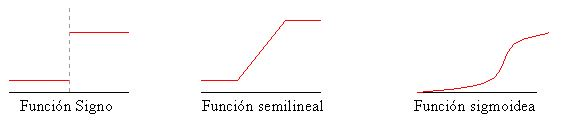
\includegraphics[width=1\textwidth]{funcionesActivacion}%
          \caption{Funciones de activación}%
          \label{figfuncionesActivacion}%
        \end{center}%
  	\end{center}%
\end{figure}%
\newpage

\subsection{Red Neuronal Artificial RNA}

Una red neuronal Artificial RNA es un grafo dirigido en el que las neuronas artificiales estas conectadas con otras y los enlaces pueden aumentar o disminuir el estado de activación de las neuronas conectadas. Cada neurona opera de forma individual mediante operaciones de suma.\cite{wiki:redesNeuronalesArtificiales}

Estas neuronas se organizan en capas o layers formando diferentes filtros para generar algoritmos que puedan resolver diferentes problemas. Dentro de una misma capa las neuronas suelen ser del mismo tipo y podemos diferenciar de forma general 3 tipos distintos de capas:

\begin{itemize}
	\item{De entrada}: Reciben datos o señales externos del entorno.
	\item{De salida}: Proporcionan las respuestas de la red ante los estímulos recibidos por las capas de entrada.
	\item{Ocultas}: No interaccionan con el entorno, son nodos intermedios que ejecutan las operaciones internas de la red.
\end{itemize}

\begin{figure}[h]
    \begin{center}%
        \begin{center}%
          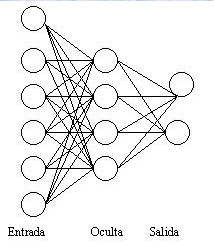
\includegraphics[width=0.7\textwidth]{RNA}%
          \caption{Grafo de una RNA}%
          \label{figRNA}%
        \end{center}%
  	\end{center}%
\end{figure}%

Como se puede observar en la figura \ref{figRNA}, las neuronas representadas como nodos se organizan en las diferentes capas pudiéndose interconectar con varias neuronas a la vez. Estas redes pueden tener un número de capas y neuronas ilimitados. Pueden tener un número ilimitado de enlaces o solo estar conectadas con unas pocas.

\newpage
\subsection{Redes neuronales convolucionales}

Este tipo de redes neuronales son muy parecidas a las RNA normales pero tienen dos cambios significativos. El primero es que parten de la idea de que las entradas son imágenes lo que permite programar optimizaciones a los algoritmos para que se adecuen a este tipo de entradas, el segundo cambio es que intentan reducir en la mayor medida posible el número de parametros utilizados en cada capa.\cite{redesNeuronalesConvolucionales}

\begin{figure}[h]
    \begin{center}%
        \begin{center}%
          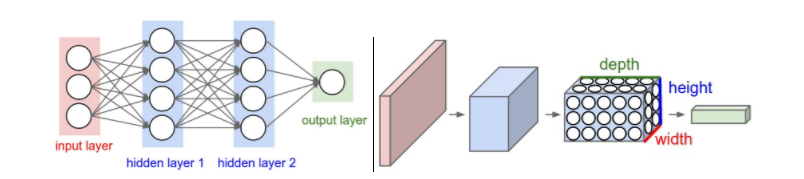
\includegraphics[width=1\textwidth]{RNAvsConvolucional}%
          \caption{Izquierda: grafo de una RNA. Derecha: Grafo de una Red neuronal convolucional.}%
          \label{figRNAvsConvolucional}%
        \end{center}%
  	\end{center}%
\end{figure}%

Las redes neuronales convolucionales organizan sus neuronas en capas de 3 dimensiones normalmente coincidiendo con las características de la imágen, siendo height la altura de la foto, width el ancho y depth los colores de la imágen. Por ejemplo se podría apicar a imágenes de 32x32x3.

\subsection{Tipos de capas}

En este apartado se van a explicar los tres tipos de capas más importantes a la hora de elabora las redes neuronales convolucionales:
%https://ccc.inaoep.mx/~pgomez/deep/presentations/2016Loncomilla.pdf
\subsubsection{Capas convolucionales}

En estas capas los pixeles de salida son combinaciones lineales de diferentes pixeles de entrada lo que generan nuevos mapas de pixeles mas sencillos y que no son tan sensibles a cambios en las entradas.\cite{redesConvolucionales} Las convoluciones se pueden producir teniendo en cuenta solo 2 dimensiones(el alto y ancho) o teniendo en cuenta las 3 dimensiones (alto, ancho y profundidad). En algunas arquitecturas son llamadas capas RELU, ejecutan la función de activación de las neuronas.

\begin{figure}[h]
    \begin{center}%
        \begin{center}%
          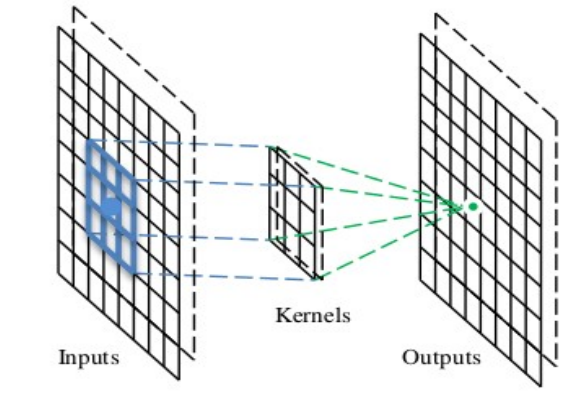
\includegraphics[width=0.7\textwidth]{convolucion}%
          \caption{Figura que muestra una convolución en dos dimensiones.}%
          \label{figconvolucion}%
        \end{center}%
  	\end{center}%
\end{figure}%
 
Como vemos en la figura \ref{figconvolucion} Los kernels definen el área sobre el que se va a aplicar la convolucion, en el ejemplo 3x3.

\subsubsection{Capas de pooling}

Las capas de pooling o reescalado tiene el objetivo de disminuir el número de parámetros o pixeles de los mapas, para ello se aplican técnicas como la explicada en la siguiente figura.

Estas capas van a tener un gran peso en los modelos de Mobilenet e Inception, ya que nos van a permitir ajustar el número de operaciones realizadas por los modelos para que se puedan ajustar correctamente a las limitaciones hardware de los teléfonos móviles.

\begin{figure}[h]
    \begin{center}%
        \begin{center}%
          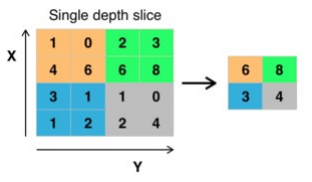
\includegraphics[width=0.7\textwidth]{pooling}%
          \caption{Técnica de máx pooling.}%
          \label{figpooling}%
        \end{center}%
  	\end{center}%
\end{figure}%

En la figura \ref{figpooling} se puede observar que los diferentes pixeles se agrupan eligiendo sólo aquellos de mayor valor para el nuevo mapa.

\subsubsection{Capas totalmente conectadas}

En este tipo de capas las neuronas están totalmente conectadas con las neuronas de la capa anterior y tienen una profundidad igual al número de clases que se quieran clasificar. Por ejemplo si tenemos 10 clases diferentes, el último layer podría se de tamaño 32x32x10. Estas capas son las encargadas de producir la señal de salida y clasificar la imagen eligiendo una de las clases. 

Cuando re entrenamos un modelo, normalmente lo que estamos haciendo es modificar estas últimas capas que se encargan de clasificar las clases en vez de tener que re entrenar todas las demás capas que forman el modelo.

\section{Modelo Inception}

El modelo Inception es una red neuronal convolucional que se usa para la clasificación de imagenes. Inception ha sido desarrollado por Google y parte de la pregunta de que tipo de convolución aplicar en cada capa o  filtro del modelo. Es decir, preguntarse que tamaño de convolución sería el adecuado para cada etapa, ¿3x3?,¿1x1?,¿5x5?.\cite{depthwiseSeparableConvolutions}

Ante esta pregunta, la respuesta que han aplicado es la de ejecutar los diferentes tamaños de convoluciones en cada capa de manera paralela y concatenar los diferentes mapas en uno solo que es el que se pasa a la siguiente capa del modelo. La idea es ejecutar todos los tipos de convulciones a la vez y elegir el que mejor funcione.

\begin{figure}[h]
    \begin{center}%
        \begin{center}%
          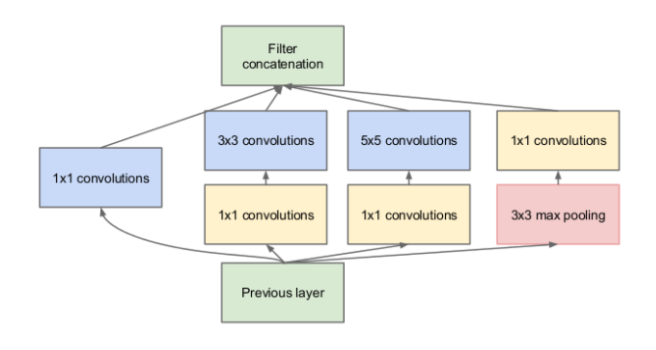
\includegraphics[width=1\textwidth]{inception}%
          \caption{Ejemplo de un nodo Inception.}%
          \label{figinception}%
        \end{center}%
  	\end{center}%
\end{figure}%

En la figura \ref{figinception} podemos observar como se aplican las diferentes convoluciones en pararelo. Además podemos observar que se aplican unas convoluciones de 1x1, estas convoluciones tienen el objetivo de reducir el número de parámetros que se usan ya que aunque no reducen el área de los mapas si reducen la profundidad de las capas.\cite{inception}

Los modelos inception se construyen concatenando estos bloques o nodos Inception, en teoría cuanta más profundidad se de a estos modelos y más se concatenen más precisos deberían ser los modelos pero esto tiene un coste alto de computación (Aún reduciendo los computos con las convoluciones 1x1) y se corre el riesgo de sobreajustar los modelos.

Actualmente se pueden entrenar diferentes versiones de Inception, en el proyecto hemos trabajado reentrenando la versión 3 del modelo mediante Tensorflow.

Este modelo se sigue desarrollando y los desarrolladores lo van evolucionando por lo que no es de extrañar que en un futuro cercano aparezcan nuevas versiones mas optimizadas de este modelo.

\begin{figure}[h]
    \begin{center}%
        \begin{center}%
          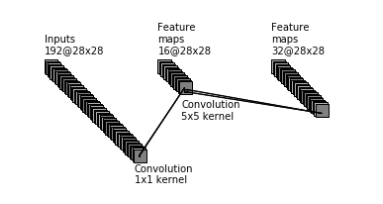
\includegraphics[width=1\textwidth]{convolicionReduccion}%
          \caption{Aplicación de una convolucion 1x1 antes de ejecutar la convolucion 5x5.}%
          \label{figconvolicionReduccion}%
        \end{center}%
  	\end{center}%
\end{figure}%

En la figura \ref{figconvolicionReduccion} se puede observar el efecto de aplicar una convolucion 1x1 antes de efectuar la convolucion 5x5.

\section{Modelo Mobilenet}

Mobilenet hace referencia a una serie de modelos clasificadores de imágenes desarrollados por Google para ser embebidos en dispositivos móviles o sistemas con pocos recursos. La filosofía de este tipo de clasificadores nace en contraposición a la tendencia que se estaba implantando en las redes neuronales de crear redes profundas y complejas con el objetivo de mejorar la precisión dejando a un lado cuestiones como el tamaño del modelo o la rapidez.\cite{mobilenet}

Los modelos Mobilenet intentan ser precisos pero a la vez ser modelos de poco tamaño y rápidos que se adecuen a sistemas que necesiten de estas ventajas, como pueden ser los automóviles autónomos, realidad aumentada, sistemas de reconocimiento, entre otros.

La arquitectura de este tipo de modelo, al igual que el modelo Inception explicado anteriormente, se basa en una red neuronal convolucional que se explicará en el siguiente apartado.

\subsection{Arquitectura Modelo Mobilenet}

La arquitectura del modelo Mobilenet se basa en dividir los filtros convolucionales típicos de una RNA totalmente conectada en dos nuevos tipos de filtros, los filtros convolucionales profundos (Del inglés Depthwise Convolutional Filters) y los filtros convolucionales puntuales (Del inglés Pointwise Convolution Filters).

El objetivo de esta división de fitros es el de minimizar el número de operaciones realizada. La convoluciones normales tienen el siguiente coste \ref{eq:convolucionNormal}:

\begin{equation} \label{eq:convolucionNormal}
	DK * DK * M * N * DF * DF
\end{equation}

DK=Tamaño del kernel (alto x ancho), M=Número de canales de entrada, N=número de canales de salida, DF=Tamaño del mapa de salida.

Los Depthwise Convolutional Filters tienen el siguiente coste computacional \ref{eq:convolutionalFilter}:

\begin{equation} \label{eq:convolutionalFilter}
	DK * DK * M * DF * DF
\end{equation}

Y los Pointwise Convolution Filters tienen el siguiente coste \ref{eq:pointwiseFilter};

\begin{equation} \label{eq:pointwiseFilter}
	M * N * DF * DF
\end{equation}

Si expresamos la convolución como un proceso de dos pasos de filtrado y combinación de los dos filtros anteriores obtenemos la siguiente reducción de costes de computación \ref{eq:convolución}:
\begin{equation} \label{eq:convolución}
(DK * DK * M * DF * DF + M * N * DF * DF)/
(DK * DK * M * N * DF * DF) = (1/N)+(1/(DK*DK))
\end{equation}

Lo que supone una reducción respecto a los filtros convolucionales normales. Esta reducción la podemos observar en la siguiente tabla:
\newpage
\tablaSmall{Depthwise Separable vs Full Convolution MobileNet}{l c c c}{herramientasportipodeuso}
{ \multicolumn{1}{l}{Modelos} & Imagenet Accuracy & Million Mult-Adds & Million Parameters \\}{ 
Conv MobileNet & 71.7\% & 4866 & 29.3 \\
MobileNet & 70.6\% & 569 & 4.2 \\
} 

Estos dos tipos de filtros se aplican de forma separada y paralela como sucedía en el modelo Inception. Para ver como surgen estas convoluciones vamos a fijarnos en la siguiente figura \ref{figconvolucionesMobilenet}.

\begin{figure}[h]
    \begin{center}%
        \begin{center}%
          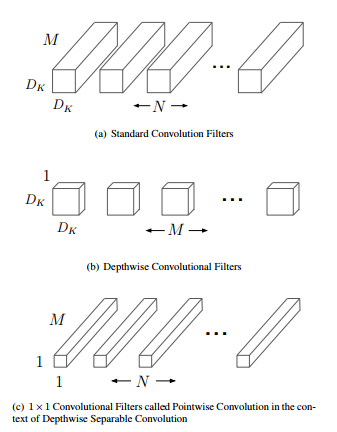
\includegraphics[width=0.7\textwidth]{convolucionesMobilenet}%
          \caption{Los filtros convolucionales normales son divididos en los filtros profundos y los puntuales.}%
          \label{figconvolucionesMobilenet}%
        \end{center}%
  	\end{center}%
\end{figure}%

El uso de estos tipos de filtros de forma paralela, más el uso de filtros de normalización y pooling, es lo que usa Mobilenet para ejecutarse de forma rápida y utilizando la menor cantidad de memoria posible.

\section{Data Augmentation}

	El Data Augmentation es una técnica que busca ampliar el conjunto de datos de entrenamiento, aplicando unas serie de transformaciones sobre las imágenes iniciales. \cite{NIPS2012_4824}
	
En las imágenes de entrenamiento se aplican una serie de técnicas como son la rotación, recortes, incremento del brillo, cambio de la gama de colores  entre otras, para conseguir nuevas imágenes que usar para el entrenamiento del clasificador.

Esta técnica nos permite ampliar nuestro conjunto de datos sin tener almacenadas estas imágenes extras a cambio de un procesamiento extra a la hora de entrenar.

Para evitar el sobreajuste del modelo, ya que estas imágenes creadas están muy interrelacionadas entre si, se ejecutan las transformaciones con una probabilidad, disminuyendo así el número de imágenes artificiales.


\section{Web Semántica}

La Web semántica es una Web extendida desarrollada bajo los estándares W3C (World Wide Web Consortium). Esta Web extendida aplica metadatos a la información que recoge para que los usuarios puedan encontrar respuestas de una manera más rápida y sencilla gracias a esta información adicional.\cite{webSemantica} 

Estos metadatos son los que otorgan más semántica a la Web y permiten obtener soluciones a problemas habituales gracias al uso de una arquitectura común para toda la información. 

Por ejemplo, en este proyecto, esta tecnología ha permitido automatizar todo el proceso de recogida de información de las diferentes especies de setas de una manera rápida y eficaz.

\subsection{¿Para qué sirve?}

A la Web actual que todos conocemos le podemos atribuir dos problemas que han surgido del enorme crecimiento que ha tenido. Estos problemas son una sobrecarga de información, mucha de la información esta repetida en diferentes lugares siendo la misma, y que la información no se muestra bajo una estructura común, sino de una forma heterogénea.

La web semántica busca solucionar estos problemas delegándolos en el software, este software es capaz de procesar su contenido, combinarlo y realizar deducciones lógicas para solucionar problemas habituales.

\subsection{¿Cómo funciona?}

El funcionamiento de la web semántica se basa esencialmente en RDF, SPARQL y OWL, mecanismos que permiten convertir la estructura de la Web para que se adecue al funcionamiento de una Web Semántica.
\begin{itemize}
	\item{RDF}: RDF permite introducir metadatos descriptivos en los distintos tipos de información.
	\item{SPARQL}: Es el lenguaje de consultas que nos permite realizar búsquedas sobre la información que contiene estos metadatos.
	\item{OWL}:OWL permite crear vocabularios para asociar los diferentes recursos.
\end{itemize}

El uso conjunto de estos mecanismos es el que nos permite razonar sobre los datos de la Web.

\section{Web Scraping}

La herramienta del Web Scraping es una herramienta para extraer información o datos de páginas web de una manera rápida, eficiente y automatizada. La información extraída se presenta de una forma más estructurada y fácil de usar.\cite{webScraping}

Los programas para realizar Web Scraping se pueden programar en diferentes lenguajes de programación, los más populares son Java, Python, Ruby y Node. Además existen diversos programas para realizar estas acciones mediante un interfaz gráfico.

Aproximadamente el 70\% de la información publicada en Internet esta en formato PDF, un formato no estructurado y difícil de manejar. Sin embargo, las páginas web si que tienen un formato estructurado ya que están programadas en código HTML, pero aun así no están presentadas de una manera totalmente reutilizable ya que no todas siguen el mismo esquema.

La técnica más extendida de Web Scraping es analizar la estructura del código HTML propio de una página web para poder extraer la información buscada. Por ejemplo, extraer todos los atributos text de los label <p> que se encuentren en una determinada página Web.


\section{Clave Dicotómica}

Las claves dicotómicas son herramientas que periten identificar organismos. Las claves pueden determinar animales, plantas, hongos,moneras, protistas o cualquier otro ser vivo. Las claves pueden alcanzar diferentes profundidades identificando el género, especie, familia, entre otros.

La clave dicotómica se basa en ir mostrando al usuario diferentes dilemas(afirmaciones contrapuestas) entre los que deberá ir eligiendo el que más se adecue al organismo a identificar hasta alcanzar la categoría taxonómica\footnote{Grupos en los que se clasifican los seres vivos.} deseada. Estas afirmaciones están enumeradas a lo largo de la clave.

\subsection{¿Cómo usar una clave?}

Usar una clave consiste simplemente en leer los diferentes dilemas y optar solamente por uno de ellos. El dilema elegido no volverá a aparecer en el desarrollo de la clave.
\cite{claveDicotomica}


































































